% ============================================================
% CAPÍTULO: RESULTADOS
% ============================================================

\chapter{Resultados}\label{sec:resultados}

Este capítulo apresenta os resultados obtidos em cada etapa do sistema desenvolvido: a segmentação binária das copas de árvores com a U-Net, a separação de instâncias individuais via algoritmo \textit{Watershed} e a classificação de espécies arbóreas com a EfficientNet-B0. Ao final, descreve-se o produto integrado do \textit{pipeline}, composto por arquivos geoespaciais com a localização e a espécie predita de cada árvore detectada.

% ------------------------------------------------------------
\section{Configuração Experimental}\label{sec:config_exp}
% ------------------------------------------------------------

Os experimentos foram realizados em um ambiente Linux com GPU NVIDIA, utilizando as bibliotecas PyTorch 2.x e \textit{segmentation\_models\_pytorch}. As imagens aéreas, capturadas em formato GeoTIFF pelo drone sobre a cidade de Rio Paranaíba -- MG, foram recortadas em \textit{tiles} de $512 \times 512$ pixels. As máscaras binárias de referência (\textit{ground truth}) foram criadas manualmente, associando cada pixel à classe \textit{árvore} (1) ou \textit{fundo} (0).

A divisão dos dados seguiu a proporção 70\% para treinamento e 30\% para validação, com seleção aleatória fixa (\texttt{random\_state = 42}) para garantir reprodutibilidade. A função de perda utilizada no treinamento da U-Net combinou a \textit{Binary Cross-Entropy} (BCE) e a \textit{Dice Loss} em partes iguais:

\begin{equation}
    \mathcal{L} = 0{,}5 \cdot \mathcal{L}_{\text{BCE}} + 0{,}5 \cdot \mathcal{L}_{\text{Dice}}
    \label{eq:loss}
\end{equation}

Essa combinação tem como objetivo equilibrar a sensibilidade a falsos negativos (Dice) com a estabilidade numérica do treinamento (BCE) \cite{jadon2020survey}. O otimizador AdamW foi empregado com \textit{weight decay} de $10^{-4}$, e o treinamento utilizou precisão mista (\textit{Automatic Mixed Precision} -- AMP) para reduzir o consumo de memória e acelerar os cálculos.

% ------------------------------------------------------------
\section{Segmentação Binária de Copas de Árvores}\label{sec:result_seg}
% ------------------------------------------------------------

A segmentação das copas de árvores nas imagens aéreas foi realizada por uma U-Net \cite{ronneberger2015u}, cujo codificador (\textit{encoder}) foi pré-treinado no conjunto ImageNet. Foram conduzidos dois conjuntos de experimentos: primeiro, uma comparação entre diferentes arquiteturas de \textit{encoder} para selecionar a mais adequada à tarefa; segundo, uma análise do impacto da resolução das imagens e das estratégias de aumento de dados (\textit{data augmentation}).

% - - - - - - - - - - - - - - - - - - - - - - - - - - - - - -
\subsection{Comparativo de Encoders}\label{sec:bench_enc}
% - - - - - - - - - - - - - - - - - - - - - - - - - - - - - -

Quatro arquiteturas de \textit{encoder} foram avaliadas em duas taxas de aprendizado distintas ($10^{-4}$ e $5 \times 10^{-5}$), mantendo os demais hiperparâmetros fixos: imagens de $512 \times 512$ pixels, \textit{batch size} de 6 e até 40 épocas com \textit{early stopping} (paciência de 5 épocas). A métrica de referência adotada foi o \textit{Intersection over Union} (IoU), também denominada Índice de Jaccard:

\begin{equation}
    \text{IoU} = \frac{|A \cap B|}{|A \cup B|} = \frac{TP}{TP + FP + FN}
    \label{eq:iou}
\end{equation}

A Tabela~\ref{tab:benchmark_encoders} apresenta o melhor IoU obtido por cada configuração no conjunto de validação.

\begin{table}[H]
    \centering
    \caption[Comparativo de encoders da U-Net]{Comparativo entre encoders para a U-Net na tarefa de segmentação binária de copas. Melhor IoU de validação por configuração de \textit{encoder} e taxa de aprendizado.}
    \label{tab:benchmark_encoders}
    \begin{tabular}{llcc}
        \toprule
        \textbf{Encoder}         & \textbf{Taxa de Aprendizado} & \textbf{Melhor IoU} & \textbf{Limiar ótimo} \\
        \midrule
        ResNet-34                & $1{,}0 \times 10^{-4}$       & 0,706               & 0,6 \\
        ResNet-34                & $5{,}0 \times 10^{-5}$       & 0,706               & 0,6 \\
        ResNet-50                & $1{,}0 \times 10^{-4}$       & 0,717               & 0,5 \\
        ResNet-50                & $5{,}0 \times 10^{-5}$       & 0,706               & 0,6 \\
        MobileNet-V2             & $1{,}0 \times 10^{-4}$       & 0,718               & 0,5 \\
        MobileNet-V2             & $5{,}0 \times 10^{-5}$       & 0,713               & 0,6 \\
        EfficientNet-B0          & $1{,}0 \times 10^{-4}$       & 0,719               & 0,7 \\
        \textbf{EfficientNet-B0} & $\mathbf{5{,}0 \times 10^{-5}}$ & \textbf{0,722}  & \textbf{0,5} \\
        \bottomrule
    \end{tabular}
    \fonte{Próprio Autor}
\end{table}

A EfficientNet-B0 com taxa de aprendizado $5 \times 10^{-5}$ obteve o melhor desempenho, alcançando IoU de $0{,}722$ com limiar de binarização de $0{,}5$. A ResNet-34 apresentou os resultados mais baixos nas duas taxas testadas ($\text{IoU} = 0{,}706$), enquanto ResNet-50 e MobileNet-V2 ficaram em posição intermediária. Apesar das diferenças absolutas serem pequenas (menos de 2 pontos percentuais), a EfficientNet-B0 demonstrou melhor equilíbrio entre capacidade representacional e custo computacional, justificando sua adoção para experimentos subsequentes de classificação de espécies.

% - - - - - - - - - - - - - - - - - - - - - - - - - - - - - -
\subsection{Impacto da Resolução e do Aumento de Dados}\label{sec:res_aug}
% - - - - - - - - - - - - - - - - - - - - - - - - - - - - - -

Além do \textit{encoder}, investigou-se o efeito da resolução das imagens de entrada e da aplicação de \textit{data augmentation} suave sobre o desempenho de segmentação. Foram realizados três experimentos principais com o \textit{encoder} ResNet-34, conforme descrito na Tabela~\ref{tab:res_aug}.

\begin{table}[H]
    \centering
    \caption[Impacto da resolução e augmentation na segmentação]{Efeito da resolução e do aumento de dados no desempenho da U-Net (encoder ResNet-34). Métricas reportadas na melhor época do conjunto de validação.}
    \label{tab:res_aug}
    \begin{tabular}{lccccc}
        \toprule
        \textbf{Configuração}         & \textbf{Res.} & \textbf{Melhor IoU} & \textbf{F1} & \textbf{Precisão} & \textbf{Recall} \\
        \midrule
        Sem augmentation              & 256 px & 0,750 & 0,857 & 0,829 & 0,888 \\
        Com aug. suave (softAug)      & 256 px & 0,722 & 0,838 & 0,809 & 0,870 \\
        \textbf{Com aug. suave (softAug)} & \textbf{512 px} & \textbf{0,749} & \textbf{0,857} & \textbf{0,831} & \textbf{0,884} \\
        Com aug. suave (softAug) -- run 2 & 512 px & 0,745 & 0,854 & 0,832 & 0,877 \\
        \bottomrule
    \end{tabular}
    \fonte{Próprio Autor}
\end{table}

As estratégias de \textit{data augmentation} empregadas foram conservadoras (\textit{softAug}): recorte aleatório com escala entre 85\% e 100\% da imagem (\texttt{RandomResizedCrop}), espelhamento horizontal com probabilidade de 50\%, e perturbações de brilho, contraste e saturação com variação de 5\% (\texttt{ColorJitter}). Optou-se por augmentações suaves porque perturbações agressivas em imagens aéreas de copas de árvores tendem a distorcer padrões de textura e forma que são discriminativos para a tarefa.

Os resultados mostram que a resolução de $512 \times 512$ pixels com augmentation suave atingiu desempenho equiparável à configuração sem augmentation em $256 \times 256$ pixels (IoU de $0{,}749$ vs. $0{,}750$), ao mesmo tempo em que contribui para maior capacidade de generalização do modelo. A aplicação de augmentation em resolução $256 \times 256$ resultou em queda de desempenho (IoU = $0{,}722$), possivelmente pelo fato de que o recorte aleatório em imagens menores elimina informações estruturais relevantes das copas.

% - - - - - - - - - - - - - - - - - - - - - - - - - - - - - -
\subsection{Evolução do Treinamento}\label{sec:curvas}
% - - - - - - - - - - - - - - - - - - - - - - - - - - - - - -

A Figura~\ref{fig:curvas_seg} apresenta as curvas de perda, F1-Score e IoU ao longo das épocas de treinamento para o melhor modelo de segmentação (ResNet-34, $512 \times 512$ px, aug. suave, $\text{lr} = 10^{-4}$). O modelo atingiu seu pico de desempenho na época 17, com IoU de $0{,}749$, precisão de $0{,}831$, \textit{recall} de $0{,}884$ e F1-Score de $0{,}857$ no conjunto de validação. A partir dessa época, observa-se estabilização das métricas de validação, sem ganhos adicionais significativos, indicando convergência adequada do treinamento.

\begin{figure}[H]
    \centering
    % INSTRUÇÃO: gerar este gráfico com matplotlib a partir de unet_metrics_512_softAug.csv
    % Sugestão: duas subplots — (1) train_loss vs val_loss por época; (2) f1 e iou por época
    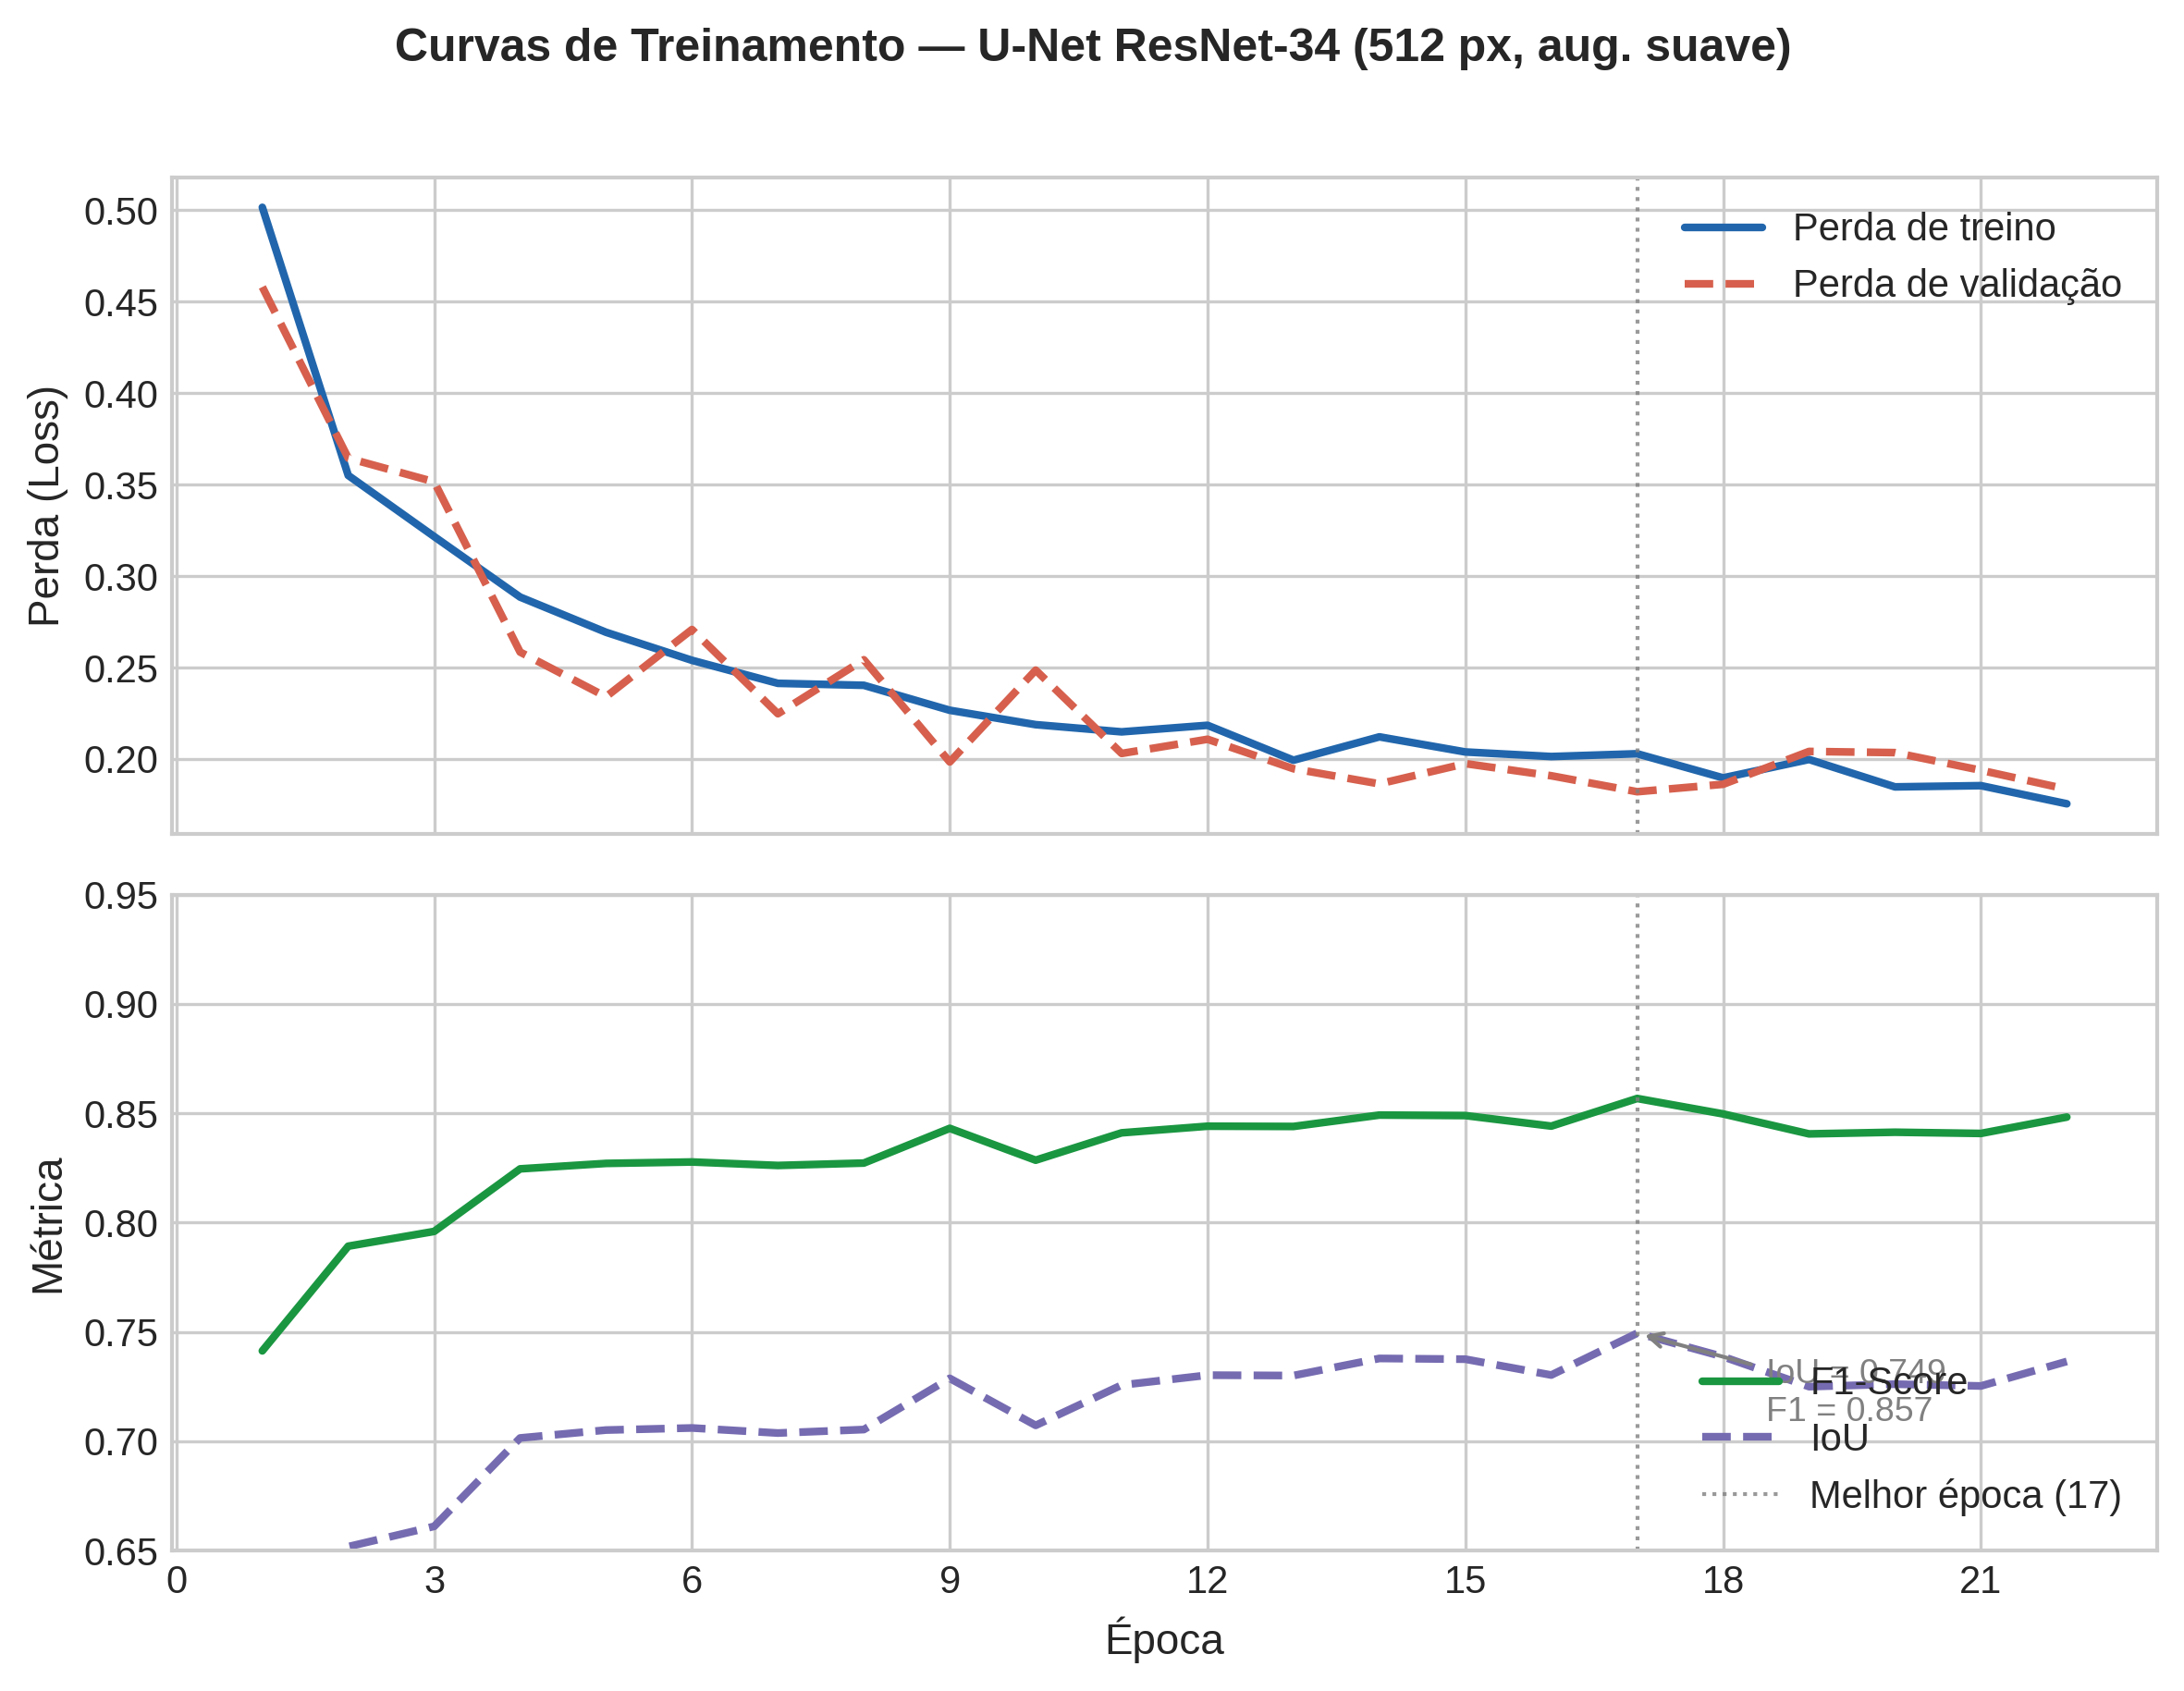
\includegraphics[width=\textwidth]{curvas_treinamento_seg.png}
    \caption[Curvas de treinamento do modelo de segmentação]{Evolução das métricas durante o treinamento do melhor modelo de segmentação (U-Net ResNet-34, $512 \times 512$ px). Acima: perdas de treino e validação. Abaixo: F1-Score e IoU de validação por época.}
    \label{fig:curvas_seg}
\end{figure}

O escalonamento automático da taxa de aprendizado (\texttt{ReduceLROnPlateau}, paciência = 3, fator = 0,5) contribuiu para a estabilidade do treinamento ao reduzir a taxa quando o IoU de validação não apresentava melhora por três épocas consecutivas. O \textit{early stopping} com paciência de 5 épocas impediu o sobreajuste nas fases finais do treinamento.

% ------------------------------------------------------------
\section{Separação de Instâncias com Watershed}\label{sec:result_watershed}
% ------------------------------------------------------------

A máscara binária produzida pela U-Net representa a área de cobertura de copa de forma agregada, sem distinguir copas individuais que se tocam ou se sobrepõem. Para individualizar cada árvore, aplicou-se o algoritmo \textit{Watershed} baseado em transformada de distância, conforme descrito a seguir.

Cada máscara binária predita passou por um pré-processamento morfológico: fechamento com disco de raio 5 pixels (\texttt{disk(5)}), remoção de pequenos buracos (limiar de área = 32 px$^2$) e remoção de objetos muito pequenos (tamanho mínimo = 32 px$^2$). Em seguida, calculou-se a transformada de distância euclidiana sobre a máscara limpa e identificaram-se os máximos locais com \textit{footprint} de $15 \times 15$ pixels como marcadores de centroide. O \textit{Watershed} foi então aplicado usando esses marcadores como sementes, delimitando regiões individuais de copa. Instâncias com área inferior a 150 pixels foram descartadas como ruído.

A Figura~\ref{fig:watershed} ilustra o processo de separação de instâncias em uma \textit{tile} de exemplo, desde a máscara binária predita até a máscara de instâncias rotuladas.

\begin{figure}[H]
    \centering
    % INSTRUÇÃO: inserir imagem comparando tile original, máscara binária e máscara de instâncias
    \includegraphics[width=\textwidth]{watershed_exemplo.png}
    \caption[Separação de instâncias com Watershed]{Exemplo de separação de copas individuais via \textit{Watershed}. Da esquerda para a direita: imagem aérea original, máscara binária predita pela U-Net e máscara de instâncias individuais após segmentação por \textit{Watershed}.}
    \label{fig:watershed}
\end{figure}

% ------------------------------------------------------------
\section{Classificação de Espécies Arbóreas}\label{sec:result_cls}
% ------------------------------------------------------------

Para cada instância de copa detectada e individualizada, extraiu-se um recorte (\textit{crop}) da imagem aérea original com margem de 16 pixels ao redor da bounding box da instância, redimensionado para $512 \times 512$ pixels. Esses recortes foram classificados por uma EfficientNet-B0 \cite{tan2019efficientnet} pré-treinada no ImageNet e ajustada para a tarefa de classificação de 6 espécies arbóreas (\textit{fine-tuning}).

O conjunto de dados de classificação foi composto por recortes anotados manualmente e por pseudorrótulos gerados automaticamente pelo próprio \textit{pipeline} (recortes com confiança de classificação superior a 0,5). Para mitigar o desbalanceamento de classes, o conjunto foi balanceado por aumento de dados (\texttt{augment\_rare\_species.py}), atingindo até 1.200 amostras para a espécie predominante e 800 amostras para cada uma das demais 5 espécies. Adicionalmente, o \texttt{WeightedRandomSampler} do PyTorch foi utilizado durante o treinamento para garantir amostragem equilibrada entre as classes a cada época.

O treinamento utilizou os seguintes hiperparâmetros: otimizador AdamW ($\text{lr} = 10^{-4}$, \textit{weight decay} = $10^{-4}$), função de perda \textit{CrossEntropyLoss}, escalonador co-ssenoidal (\texttt{CosineAnnealingLR}, $T_{\max} = 10$) e \textit{early stopping} com paciência de 5 épocas, com seleção do melhor modelo pelo F1-Score macro no conjunto de validação (divisão 80\%/20\%, estratificada por espécie).

A Tabela~\ref{tab:result_cls} apresenta as métricas obtidas pelo melhor modelo de classificação no conjunto de validação.

\begin{table}[H]
    \centering
    \caption[Métricas do classificador de espécies EfficientNet-B0]{Desempenho do classificador de espécies arbóreas (EfficientNet-B0) no conjunto de validação. Métricas calculadas com média macro entre as 6 classes.}
    \label{tab:result_cls}
    \begin{tabular}{lc}
        \toprule
        \textbf{Métrica}    & \textbf{Valor} \\
        \midrule
        Acurácia            & % TODO: preencher com o valor real do log de treinamento \\
        F1-Score (macro)    & % TODO: preencher com o valor real do log de treinamento \\
        \bottomrule
    \end{tabular}
    \fonte{Próprio Autor}
\end{table}

% INSTRUÇÃO: substituir os % TODO acima pelos valores reais obtidos no terminal ao rodar
% train_species_efficientnet.py. A saída final imprime:
%   "Melhor F1 obtido: X.XXXX"
% Adicionar também a matriz de confusão como figura, se disponível.

A Figura~\ref{fig:matriz_confusao} apresenta a matriz de confusão do classificador, evidenciando as espécies com maior taxa de acerto e aquelas com maior confusão entre classes.

\begin{figure}[H]
    \centering
    % INSTRUÇÃO: gerar a matriz de confusão durante a avaliação do modelo e exportar como imagem
    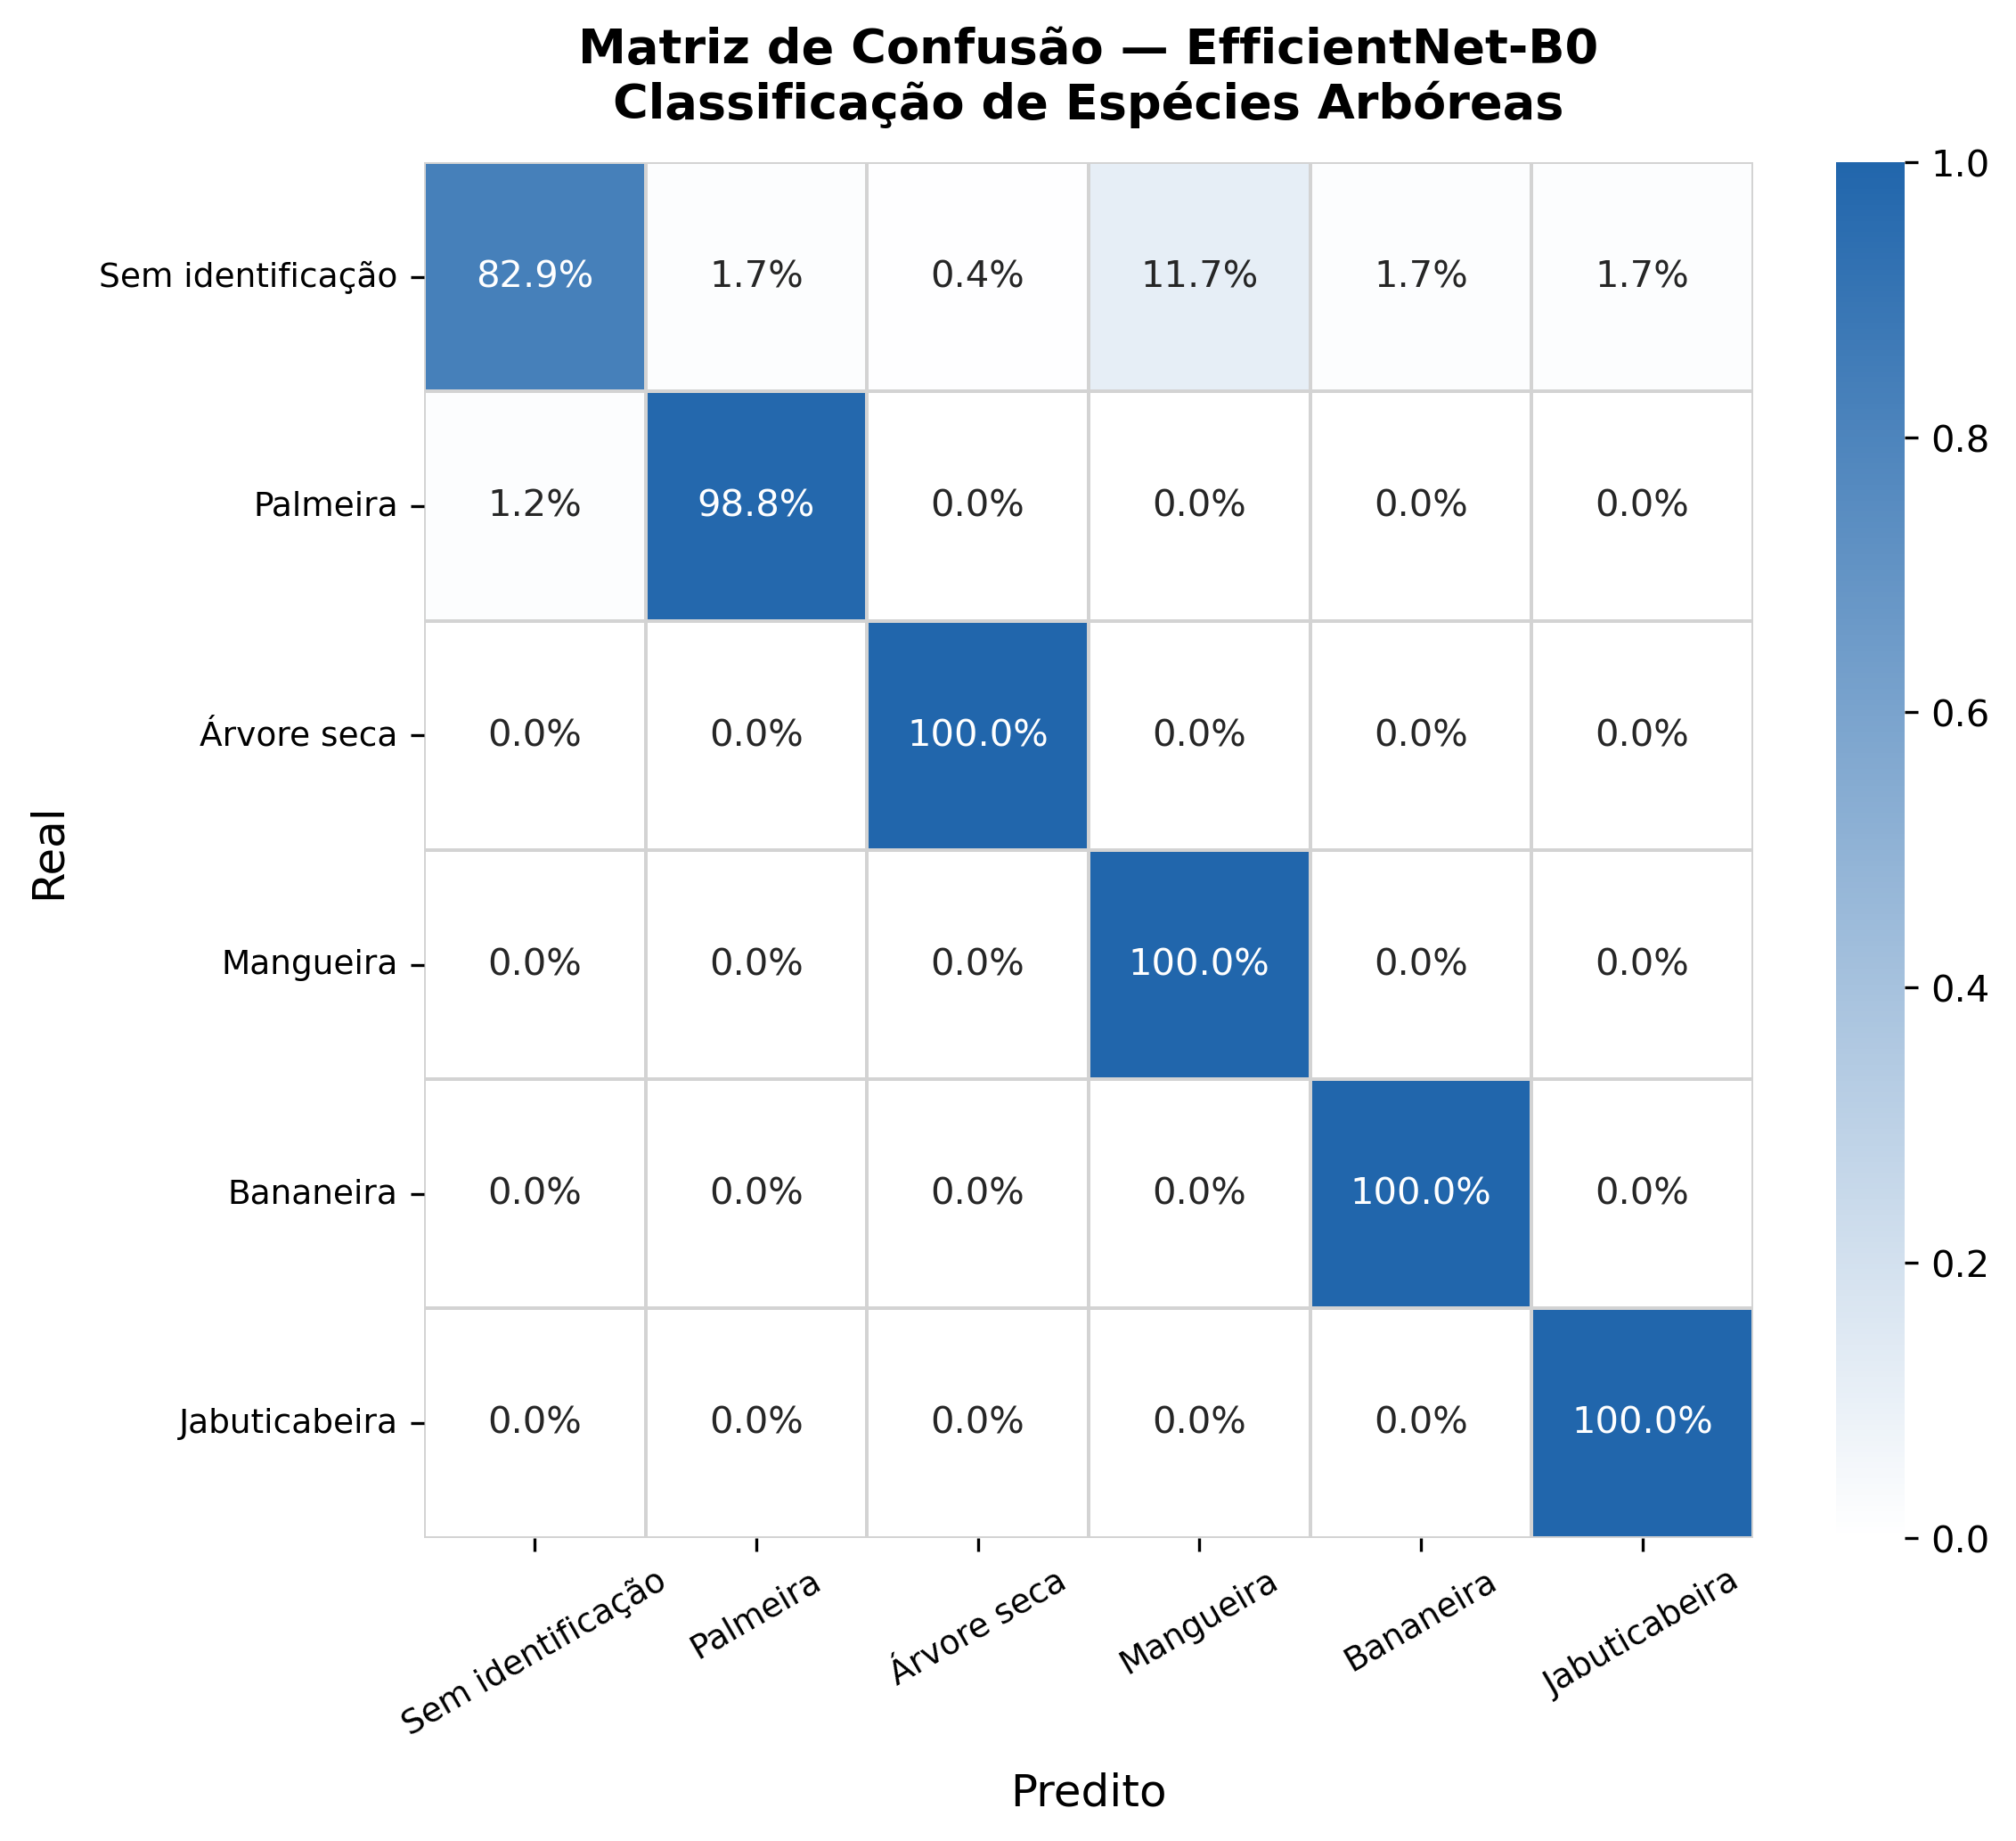
\includegraphics[width=0.75\textwidth]{matriz_confusao_especies.png}
    \caption[Matriz de confusão do classificador de espécies]{Matriz de confusão do classificador EfficientNet-B0 no conjunto de validação para as 6 espécies arbóreas identificadas em Rio Paranaíba -- MG.}
    \label{fig:matriz_confusao}
\end{figure}

% ------------------------------------------------------------
\section{Pipeline Integrado e Saída Geoespacial}\label{sec:result_pipeline}
% ------------------------------------------------------------

O \textit{pipeline} completo integrou as etapas de segmentação (U-Net), separação de instâncias (\textit{Watershed}) e classificação de espécies (EfficientNet-B0), gerando como produto final arquivos geoespaciais nos formatos GeoPackage (.gpkg) e GeoJSON. Cada instância de árvore detectada é representada como um polígono georeferenciado com os seguintes atributos: espécie predita (\texttt{predicted\_species}), confiança da predição (\texttt{confidence}), área da copa em metros quadrados (\texttt{area\_m2}), \textit{tile} de origem (\texttt{tile}) e identificador da instância (\texttt{instance\_id}).

Para lidar com instâncias duplicadas geradas em regiões de sobreposição entre \textit{tiles} adjacentes, aplicou-se o algoritmo DBSCAN sobre as coordenadas centroides das instâncias. Instâncias a menos de 2 metros entre si foram agrupadas e representadas por uma única entrada no arquivo de saída, mantendo a predição de maior confiança.

A Figura~\ref{fig:mapa_resultado} apresenta uma visualização dos resultados no ambiente QGIS, exibindo as copas segmentadas e classificadas sobre a ortofoto da área urbana de Rio Paranaíba.

\begin{figure}[H]
    \centering
    % INSTRUÇÃO: exportar visualização do GeoPackage no QGIS com legenda de espécies
    \includegraphics[width=\textwidth]{mapa_resultado_especies.png}
    \caption[Mapa de árvores detectadas e classificadas em Rio Paranaíba]{Resultado do \textit{pipeline} de detecção e classificação de árvores urbanas sobre a ortofoto de Rio Paranaíba -- MG. Cada polígono representa uma copa detectada, com cor correspondente à espécie predita pelo modelo.}
    \label{fig:mapa_resultado}
\end{figure}
